\documentclass[12pt,hyperref,a4paper,UTF8]{ctexart}
\usepackage{HDUReport}
\usepackage{listings}
\usepackage{xcolor}
\usepackage{graphicx}
\usepackage{setspace}
\usepackage{float}
\setstretch{1.5} % 设置全局行距为1.5倍

\usepackage{enumitem} % 载入enumitem包以便自定义列表环境
\setlist[itemize]{itemsep=0pt, parsep=0pt} % 设置itemize环境的项目间距和段落间距

\setmainfont{Times New Roman} % 英文正文为Times New Roman


\usepackage{tikz}
\usetikzlibrary{shapes.geometric, arrows}
\usetikzlibrary{positioning, arrows.meta}
\usetikzlibrary{calc}
%封面页设置
{   
    %标题
    \title{ 
        \vspace{1cm}
        \heiti \Huge \textbf{《电磁波与电磁场实验》作业报告} \par
        \vspace{1cm} 
        \heiti \Large {\underline{实验二:集总参数元件滤波器的设计、 仿真、调谐与优化}   }     
    }

    \author{
        \kaishu\Large 指导教师\ \dlmu[9cm]{吴爱婷}  \\
        \kaishu\Large 学生姓名\ \dlmu[9cm]{陈文轩} \\ %学院
        \kaishu\Large 学生学号\ \dlmu[9cm]{23040447} \\ %
        \kaishu\Large 学生班级\ \dlmu[9cm]{23186011} \\ %班级
        \kaishu\Large 学生专业\ \dlmu[9cm]{智能硬件与系统(电子信息工程)} \qquad  \\ %学号
        \kaishu\Large 实验日期\ \dlmu[9cm]{2025.10.13} \qquad \\
         %姓名 
    }
        
    \date{\today} % 默认为今天的日期，可以注释掉不显示日期
}
%%------------------------document环境开始------------------------%%
\begin{document}

%%-----------------------封面--------------------%%
\cover
\thispagestyle{empty} % 首页不显示页码
%%------------------摘要-------------%%
%\newpage
%\begin{abstract}




%\end{abstract}

%\thispagestyle{empty} % 首页不显示页码

%%--------------------------目录页------------------------%%
% \newpage
% \tableofcontents
% \thispagestyle{empty} % 目录不显示页码

%%------------------------正文页从这里开始-------------------%
\newpage
\setcounter{page}{1} % 让页码从正文开始编号

%%可选择这里也放一个标题
%\begin{center}
%    \title{ \Huge \textbf{{标题}}}
%\end{center}

\section{实验目的}

1.通过此次实验，熟悉集总参数滤波器软件仿真过程，熟悉MWO2010的各种基本操作。

2.本次实验我们需要用到MWO2010的优化和Tune等工具，要求熟练掌握MWO提供的这些工具的使用方法和技巧。


\section{实验内容}

采用集总参数元件设计高通滤波器；在$f>1000MHz$时，$S_21>-1db,S_11<-20db$；在$f<700MHz$时，$S_21<-30db$；仿真步长10MHz，范围100MHZ至200MHZ;要求电路对称，端口阻抗50欧姆，电路阶数为7阶。


\subsection{主要实验步骤}

1.对应题目要求，在optimizer goal中，设计填入优化目标，使程序按此方向自动优化

\begin{figure}[H]
  \centering
  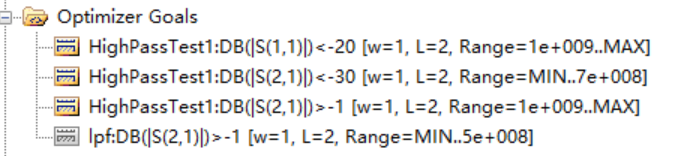
\includegraphics[width=0.8\textwidth]{figures/约束设计.png}
  \caption{优化目标设计}
  \label{fig:example}
\end{figure}

2.在优化器中，应当去除不必要的约束，才能进行较好的优化；同时对与优化目标，应当适当的加强（比如在$f<700MHz$时，改为$S_21<-35db$），这样可以更加的接近预定目标。

\begin{figure}[H]
  \centering
  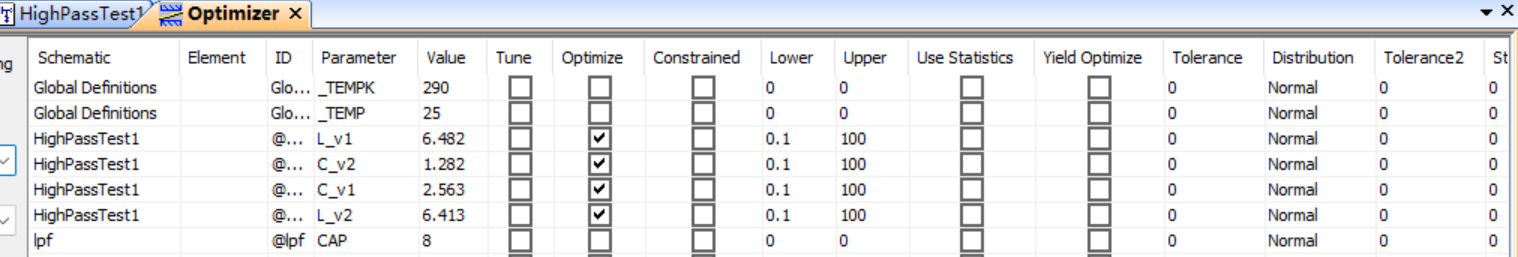
\includegraphics[width=0.8\textwidth]{figures/优化参量.png}
  \caption{优化参量设计}
  \label{fig:example}
\end{figure}

3.同时检查电路，变量与器件的绑定是否对称，检查后对称才继续优化。

\begin{figure}[H]
  \centering
  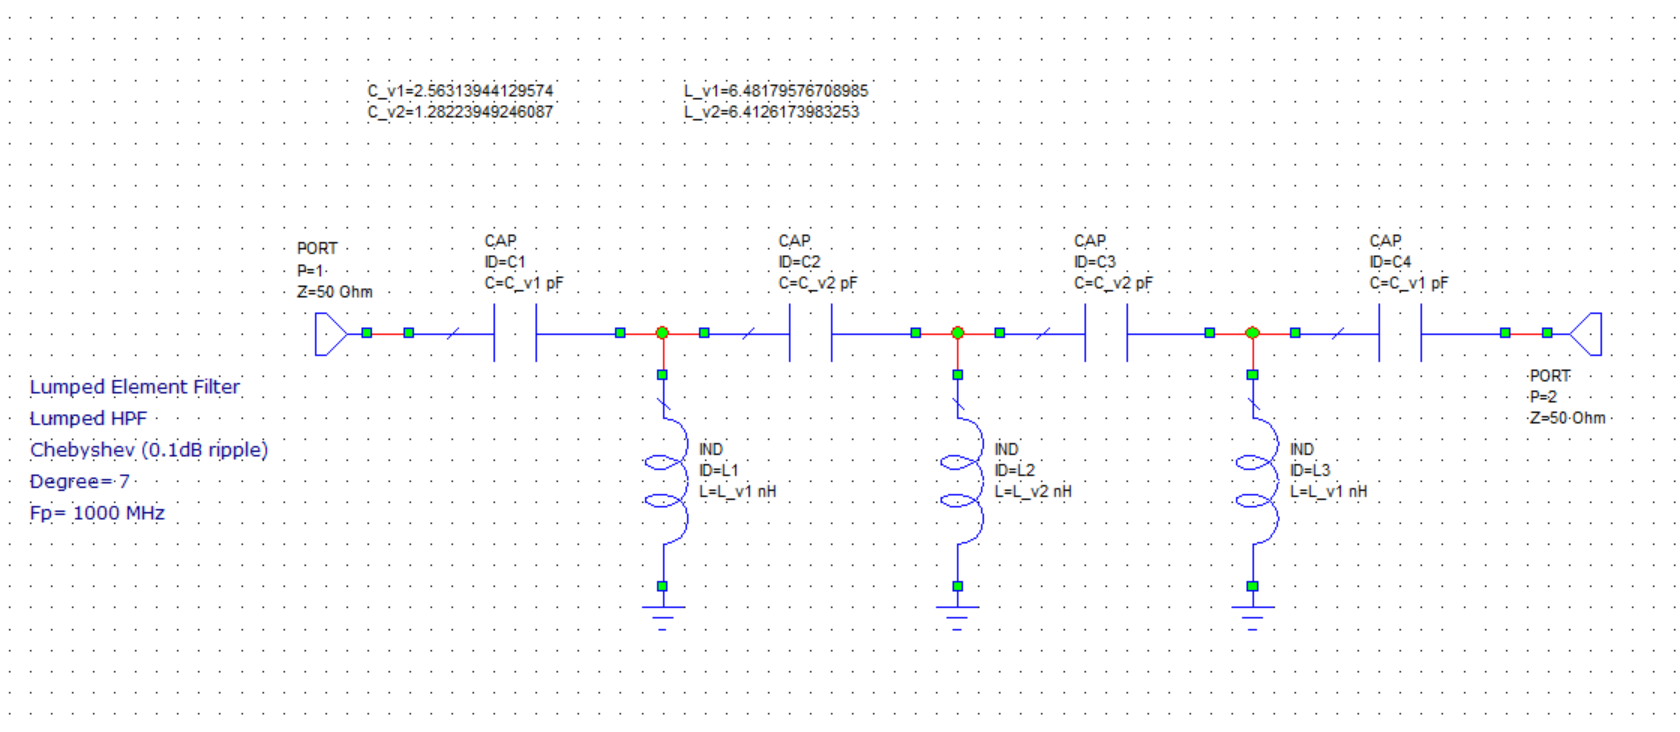
\includegraphics[width=0.8\textwidth]{figures/电路.png}
  \caption{电路与参数自动优化设计}
  \label{fig:example}
\end{figure}


4.经过多次优化调整，最后的$S_11,S_21$图像能够达到预定要求。

\begin{figure}[H]
  \centering
  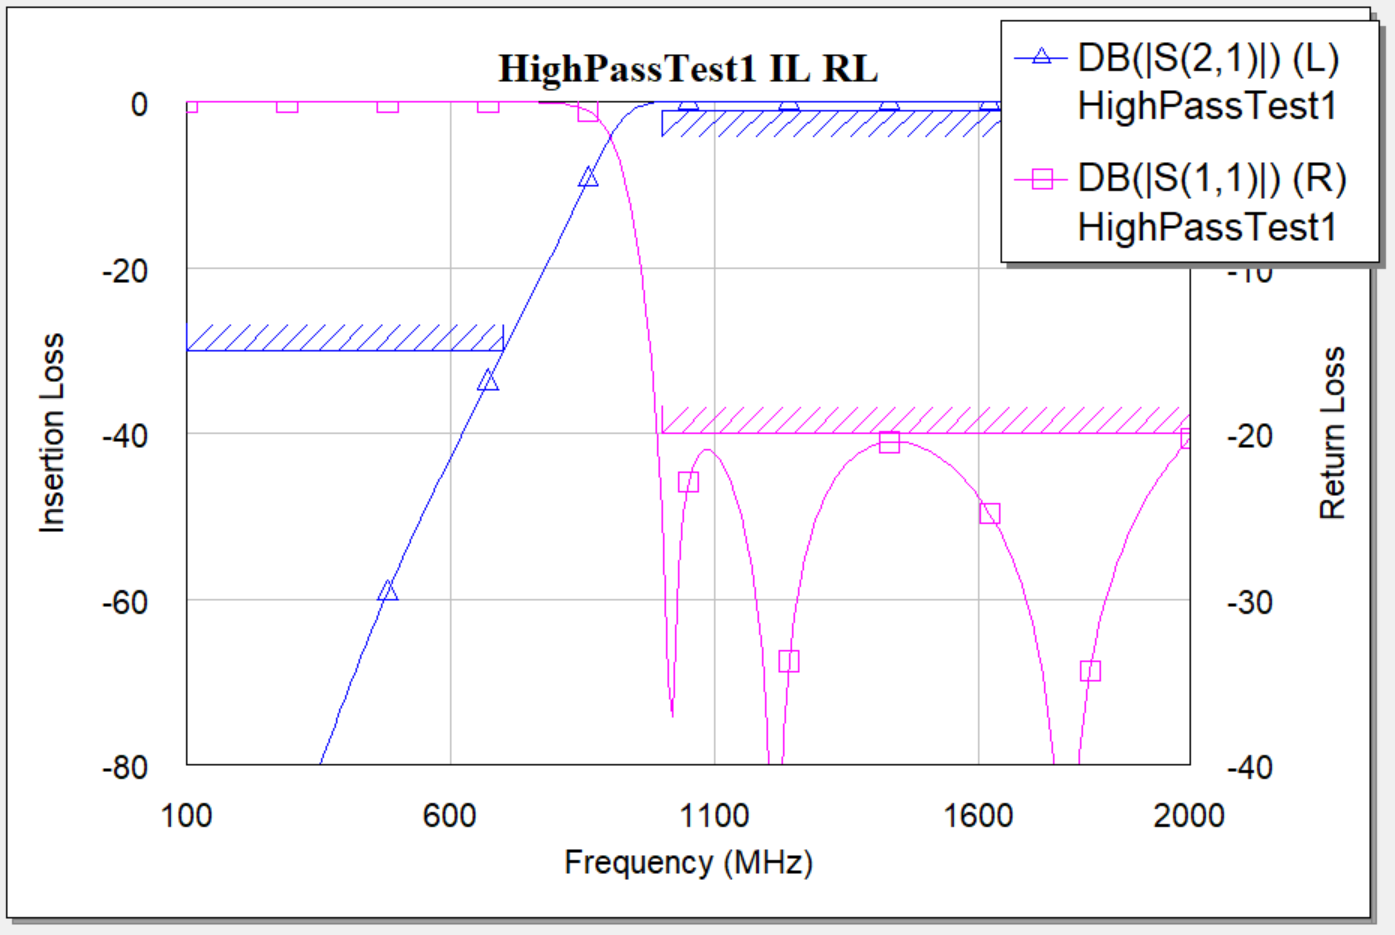
\includegraphics[width=0.8\textwidth]{figures/实验结果.png}
  \caption{实验结果}
  \label{fig:example}
\end{figure}

\section{总结}

通过本次实验，我初步掌握了使用AMR软件设计和仿真集总参数滤波器的基本流程。我学习了如何根据给定的技术指标（如通带、阻带、回波损耗等）来设定优化目标，并利用软件的优化器功能自动调整元件参数，最终使滤波器性能达到设计要求。这个过程加深了我对滤波器理论知识的理解，特别是切比雪夫滤波器的特性。

实验过程中遇到的主要困难在于优化目标的设定与优化参数的选取。起初，直接按照指标（例如 $S_{21} < -30\text{dB}$）进行优化，效果并不理想，收敛速度慢且结果难以达标。后来通过适当“加强”约束（如将目标设为 $S_{21} < -35\text{dB}$），并仔细检查电路的对称性，确保变量绑定正确，优化过程变得更加高效，最终得到了满意的仿真结果。这让我认识到，仿真设计不仅是理论的直接应用，也需要根据实际情况灵活调整策略。

关于电路中各元件对 $S_{11}$ 和 $S_{21}$ 的影响，我的理解如下：

对于一个高阶滤波器，所有元件共同决定了其整体响应，它们相互关联，共同构成了滤波器的频率选择特性。不过，不同位置的元件其影响的侧重点有所不同。

\begin{itemize}
    \item \textbf{对 $S_{21}$ (传输特性) 的影响}: 串联电容（C1, C2, C3, C4）是构成高通滤波器的核心，它们主要负责阻断低频信号、通过高频信号，其容值共同决定了滤波器的截止频率和通带形状。并联电感（L1, L2, L3）则为低频信号提供了到地的通路，极大地增强了阻带的衰减特性。因此，所有电容和电感都对 $S_{21}$ 的曲线形态有显著影响。

    \item \textbf{对 $S_{11}$ (反射特性) 的影响}: $S_{11}$ 主要反映了滤波器端口与 50 欧姆传输线的匹配程度。其中，\textbf{最靠近输入/输出端口的元件（即 C1, L1 和 C4, L3）对 $S_{11}$ 的影响最为显著}。这些元件直接构成了滤波器的输入和输出阻抗接口。它们的数值稍有偏差，就会导致端口阻抗失配，从而使得反射增大（即 $S_{11}$ 恶化）。相比之下，处于电路中心的元件（如 L2, C2, C3）虽然也影响整体匹配，但其作用更多地体现在对通带内的波纹形状和整体响应的微调上，对端口匹配的直接影响小于两端的元件。
\end{itemize}



\end{document}